\documentclass[sigconf]{acmart}
\usepackage{listings}
\usepackage{hyperref}
\usepackage[pdf]{graphviz}
\begin{document}

\title{Pennant Lines: An Alternative to Finger Trees in Dynamic Environments}

\author{Daniel Jay Haskin}

\acmConference[ELS '25]{European Lisp Symposium}{May 15--23,
  2025}{Vienna, Austria}
\email{dan@djhaskin.com}
\renewcommand{\shortauthors}{Haskin}

\begin{abstract}
Pennant Lines are presented, a novel data structure for storing persistent
sequences in Common Lisp suitable as a drop-in replacement for normal lists, but
with much better runtimes for most operations. These sequences support at least
logarithmic time when implementing a version of the Common Lisp Sequences API
persistently, and better time in other key cases. All are simpler to implement
within a dynamic setting such as that of Common Lisp than Finger Trees, and play
nicer with the larger Lisp ecosystem.
\end{abstract}

%% https://dl.acm.org/ccs.cfm
\begin{CCSXML}
<ccs2012>
<concept>
<concept_id>10003752.10003809.10010031</concept_id>
<concept_desc>Theory of computation~Data structures design and analysis</concept_desc>
<concept_significance>500</concept_significance>
</concept>
</ccs2012>
\end{CCSXML}
\ccsdesc[500]{Theory of computation~Data structures design and analysis}
\keywords{lisp, datastructure, sequences, dynamic, untyped}

%%\begin{teaserfigure}
%%  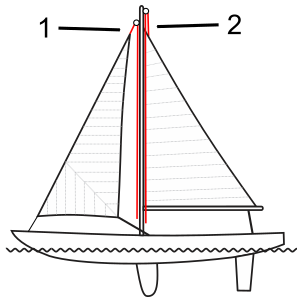
\includegraphics[width=\textwidth]{img/Halyard}
%%  \caption{A depiction of a Halyard[1].}
%%  \Description{A drawing of a sailbosat with the main and jib halyards
%%    highlighted.}
%%  \label{fig:teaser}
%%\end{teaserfigure}

%%\received{20 February 2007}
%%\received[revised]{12 March 2009}
%%\received[accepted]{5 June 2009}
\maketitle

\section{Motivation}

When in a dynamically typed language like Lisp, it is often convenient to work
with a data structure in specific ways in one moment, such as for operating on
sets, and then perform simple list operations on them the next. Alists are nice
because at the end of the day, "they are just lists" -- they can be fed into
functions that expect an array of items, like \texttt{print}. Object type is
fluid in Lisp, as is object purpose. In Lisp, data structures can be used for
their characteristics and ergonomics, rather than for their intended type. Lisp
is a highly dynamic environment.

In the dynamic environment of Common Lisp, lists are used for
\emph{everything}, from dictionaries to sets to arrays. All the tooling works
better with these data structures than with anything else. Getting the nth
element, performing set union or intersection, stack operations, and syntax
abstractions on lists are all defined in the Common Lisp standard.

However, lists present poor run time characteristics when used for anything more
complicated than a stack. Often lists are used simply because of their ease of
use with little regard for runtime. This is fine until the runtime becomes
important; then ergonomics is sacrificed and the code is rewritten data
structures which are faster, but less ergonomic.

In this presentation, we will implement a data structure with an API that imitates
the Common Lisp list API but in a way that is ergonomic, persistent by default,
and dynamic. This means the resulting data structure must be usable as a list
first, but sometimes also as a set or dictionary. By implementing functions
that mirror the list API, we make it easy for people to use the structure, since
all the functions they are used to using with lists exist and work just as they
do for lists, they just exist in a different package.

As a first attempt at this task, Finger Trees \cite{Hinze-Paterson:FingerTree}
were first examined. Finger Trees are easy
to implement in Haskell, with its algebraic sum types and pattern matching. The
problem is that they are clunky to implement in a dynamically typed language
like Lisp. Implementing Finger Trees involves polymorphic recursion. Every level
in a finger tree contains deeper 2-3 trees than the level above it, and values
are only at the leaves. The spine of the tree is different than the leaves.

This creates a lot of case-by-case work in Lisp. The CLOS is well designed, but
can be slow, especially in the "hot path" in which data structure operations
often find themselves. Without using the CLOS, we are left with the choice of
using \texttt{defstruct} and \texttt{typecase}, both of which greatly complicate
the implementation.

It would be ideal if the data structure were relatively homogeneous -- it looked
the same throughout. This would greatly decrease case logic.
%% We also want structure that is cons-based. That way, it is still "just a list"
%% and can work with a lot of list tooling --
%$% \texttt{destructuring-bind}, \texttt{copy-tree}, \texttt{tree-equal},
%% \texttt{print}, etc.

Finally, we need a structure that is tolerant to and implements functionality
for non-persistent updates along side the persistent ones. This mirrors how
lists are used in Common Lisp -- persistent by default, but changeable if need
be.

So, we need to create a data structure that is relatively homogeneous, with
few cases to manage. It must be able to be used dynamically for different
purposes. It must be persistent by default, but changeable if needed. It should
have good running time. Finally, its API should closely mirror the Common Lisp
Standard's List API.

\section{Development}

In this section we first lay out the API that needs to be implemented and summarize
what functionality needs to exist for that API. We then develop an answer to
that API with weight-balanced binary trees. Finally, develop even better run
times by adding pennant lines to the mix.

\subsection{The List API}

The Common Lisp Standard's API for lists\cite{ANSI:1994:DPA} outlines three
basic uses for conses (among others):

\begin{enumerate}
    \item As sequences of items (speaking of "proper lists").
    \item As association structures.
    \item As sets.
\end{enumerate}

We will also seek to make a datastructure suitable for these three uses using a
persistent-by-default structure. Therefore, the following operations need to be
supported:

\begin{itemize}
    \item Efficient random insertion, deletion, and access, particularly at the
        ends
    \item Efficient reduction (using a \texttt{reduce}-like function)
    \item Efficient concatenation
    \item Efficient splitting / subsequencing
    \item Efficient set operations
\end{itemize}

These will be used separately or in combination depending on the API function in
which it is used.

Then we implement the API on top of these basic operations, which will support
sets, associative structures, and plain sequences of objects.

\subsection{Observations about Ranked Binary Trees}

We first note that the Hinze and Paterson's Finger Tree ``monoid
trick''\cite{Hinze-Paterson:FingerTree} can actually be done with any tree,
including a binary search tree.

\begin{lstlisting}[caption={Our indexed binary tree type.}, label={lst:treestruct}, language=Lisp]
;;; Indexed node within a binary tree.
(defstruct node
    value
    size
    left
    right)
\end{lstlisting}

Throughout the rest of this paper, when discussing binary trees, we will use
the definition in listing \ref{lst:treestruct}.

Suppose each node in a binary search tree has also a `size` component. Then,
provided an index into the tree, insert, delete, and access operations can
be done without comparing values in the tree to each other by instead comparing
tree and subtree sizes to the currently given index. In this way, a value
can be inserted, deleted, or accessed at the given index in logarithmic time.

The access algorithm is straightforward. The index is compared against the size
components of the left and right child of the root. If the left child's size
is greater than the index, insertion recurses into the left child using the same
index. If the index equals the left child size, the value of the root node is returned.
If it is greater than the left child size, insertion recurses into the right
child using \texttt{(- index 1 (node-size (node-left tree)))} as the index.

Insertion works by finding the indexed node, swapping the value at that spot
with the value that needs inserted, and then recursing into the right child with
the swapped out value and an index of 0, followed by a rebalancing step going
back up the tree.

Deletion works by finding the indexed node, deleting the value at that spot,
then, deleting the value from the right child at index 0 (or the left child at
index \texttt{(-1 (node-size left-child))} and placing that value in the spot
which we leave behind, rebalancing as we go.

That gives us a logarithmic baseline for insertion, random access, deletion and
stack-based traversal. We still need concatenation, splitting, and set
operations. For concatenation and splitting, we can use the work due to Guy E.
Blelloch, Daniel Ferizovic, and Yihan Sun\cite{10.1145/3512769}. We'll also use
their work a bit later for set operations\cite{DBLP:journals/corr/BlellochFS16}.

We choose, then, to use "normal" binary trees as the
basis of our new data structure, instead of 2-3 leaf trees. That way, the data
structure is much more homogeneous; the code becomes simpler, with fewer cases.

Binary trees will give us a nice baseline of logarithmic time for many
operations, but if we want efficient insertion at the beginning and end, we will
have to use a Zipper\cite{HUET_1997}, kind of like Hinze and
Patterson\cite{Hinze-Paterson:FingerTree} did with Finger Trees. That means
there will be added polymorphism and hence complexity, but it will not be too
much.

\subsection{Sorted Mode: Speeding Up Set Operations}

Binary trees are a good basis for our use case for another reason: there's
nothing stopping us from treating these trees as "normal sorted sets" like the
ones that are customarily kept inside trees (rather than sequences). Operating
in a different mode on the same data structure, we could treat these "sequences"
like sets, or these "sets" like sequences. In one mode, we insert by index; in
another mode, we insert using a sort function that finds its way through the
tree by comparing the given value to insert with its compatriots in the tree.
This information could be given at runtime, using a \texttt{:sortfn <fn>}
argument instead of an \texttt{:index <ind>} to one of our functions that
operate on these pennants. Indexed binary search trees can be treated as a
set or a sequence fluidly.

When we insert, we provide a sort function instead of an index, and say that
$<=$ is used for inserting into the left child instead of $<$, now we just have
a "normal" multiset that can be merged using Guy Blelloch's stuff. We could
also take an unsorted thing and run `sort` on it and that gives a new sequence
that's sorted and immediately usable in "sorted mode".

Further, if a \texttt{:sortfn <fn>} were given to some e.g. set operation
function in our API, and was used throughout the life of the data structure, we
could then treat the tree like an ordered set and use the set operations
provided in \cite{DBLP:journals/corr/BlellochFS16} instead of treating the trees
like fancy lists when implementing the set operations. If \texttt{:sortfn}
parameter is not given, we may assume the tree is unordered, and we will just
treat the trees like normal unordered sequences when performing set operations.

\subsection{Picking the Binary Tree Balancing Algorithm}

We have one more detail to add before our baseline can be complete, though. We
must select a balancing algorithm for the tree.

We select weight balanced trees. Weight-balanced trees were originally presented
due to J. Nievergelt and E. M. Reingold\cite{doi:10.1137/0202005}, but most
recently to Y. Hirai and K. Yamamoto\cite{HIRAI_YAMAMOTO_2011}. The advantage of
weight balanced trees is that height of the trees are kept track using the size
element, something the design already requires.

The drawback is that height is
roughly kept track of effectively using the most significant bit of the size of
the tree. Thus, the ``taller'' the tree, the more bits are needed to represent
size and overflows may occur. This is fine though, since we're in Common Lisp,
since its numerical tower prevents all of that. Also, a tree of height e.g. 50
is of roughly of size $2^48$ to $2^52$ with Hirai and Yamamoto's $<3,2>$ Weight
Balanced Trees. This is both large enough to have few if any applications, but
it is also small enough to fit in the mantissa of a 64-bit floating point
integer. This means this strategy would work in most places, even in
math-constrained ones like Janet\cite{Janet} or JavaScript.

The other disadvantage is that integer multiplication is needed to get weights
to balance, but with the parameters given by Hirai and Yamamoto it is a simple
arithmetic shift followed by an addition (multiply by $3$) for $\Delta$ and a
simple arithmetic shift for $\Gamma$, so that's not a problem either. (In 64-bit
float languages, it's an increment of the exponent and addition or simply
exponent increment, and is equally easy to do.)

(Draft note, primer for WB trees goes here in the actual paper)

\subsection{Concatenation and Splitting}

We have at least a logarithmic baseline for insertion, deletion, and access
within our sequence.

Next we have concatenation and splitting to consider.

%%Guy Blelloch et. al. gave us fantastic recipes for merging and splitting
%%trees _where a middle key is already present_, but if we have two trees together,
%%and we wished to merge them (thus concatenating the list), we would have to
%%delete the maximum element from one tree or the minimum from the other,kkkk
%%resulting in logarithmic time concatenation or splitting, even if two
%%trees are of equal size.
%%
%%Seeking to ensure that, if two trees are of equal size, merging and splitting
%%takes $O(1)$ time, we observe that if we already \emph{had} a pivot element, it
%%would be $O(1)$ time. So, we should make sure we always have a pivot element
%%handy.k
%%
To this end, we next consider a tree where:

1. The root has no left child
2. The right child is an arbitrarily large balanced binary tree

We first start with a complete tree:

\digraph{CompleteTree}{
    size="2.5,3";
    node[shape=box];
    subgraph pivot {
        0;
    }
    subgraph left {
        a;
        b;
        c;
        d;
        e;
        f;
        g;
        a -> b;
        a -> c;
        b -> d;
        b -> e;
        c -> f;
        c -> g;
    }
    subgraph right {
        2 -> 1;
        2 -> 3;
        4 -> 2;
        4 -> 6;
        6 -> 5; 
        6 -> 7;
    }
    0 -> a;
    0 -> 4;
}

Then we break the left side off:

\digraph{BrokenTree}{
    size="2.5,3";
    node[shape=box];
    subgraph pivot {
        0;
    }
    subgraph left {
        a[style=invis];
        b[style=invis];
        c[style=invis];
        d[style=invis];
        e[style=invis];
        f[style=invis];
        g[style=invis];
        a -> b[style=invis];
        a -> c[style=invis];
        b -> d[style=invis];
        b -> e[style=invis];
        c -> f[style=invis];
        c -> g[style=invis];
    }
    subgraph right {
        4 -> 2;
        4 -> 6;
        2 -> 1;
        2 -> 3;
        6 -> 5; 
        6 -> 7;
    }
    0 -> a[style=invis];
    0 -> 4;
}

We end up with a pennant tree whose first node is the "minimum" knode, the one
that comes first in the sequence. It could be rendered thus:

\begin{figure}
    \caption{A complete pennant tree.}
    \label{complete-pennant}
    \digraph{PennantTree}{
        size="2.5,3";
        node[shape=box];
        subgraph pivot {
            0;
        }
        subgraph right {
            4 -> 2;
            4 -> 6;
            2 -> 1;
            2 -> 3;
            6 -> 5; 
            6 -> 7;
        }
        0 -> 4;
    }
\end{figure}

In the above illustration, we have a sequence of 8 spots, with each spot labeled
with its relative index in a list.

To make a pennant tree $P$, we simply keep a pair of things. The first member of the
pair is $m$ the minimum node, and the second member $t$ is the "rest" of the
tree, the part of the pennant that is a normal binary search tree:

\begin{equation}
    P = <m,t>
\end{equation}

By always carrying around an explicit minimum element $m$, concatenation and
splitting of two trees of equal size stays in constant time.

Given two trees $Q = <m_q,t_q>$ and $R = <m_r,t_r>$, we construct a new tree $S
= <m_q,j(t_q, m_r, t_r)>$, where $j(l,p,r)$ creates a new tree by joining
balanced trees $l$ and $r$ using pivot $p$.

Similarly, given a tree $S = <m_s,t_s>$, we simply reverse the operation. We
take the pivot element $p$ of $t_s$, and its left and right branches $l$ and
$r$, and construct two new trees $Q = <m_s, l>$ and $R = <p, r>$ out of their
parts.

Merging and splitting two trees of unequal size is easy as well, and is described in
\cite{10.1145/3512769}.

For merging, assume we have two trees representing sequences, $a$ and
$b$, with the elements of $a$ coming before those of $b$.

Assume that $a$ is the larger tree. Then we traverse down the \emph{right spine}
of $a$, always choosing the right child as we traverse, until we find a tree
that is "roughly" of equal size. We decide this by checking if the subtree of
$a$ is balanced with $b$. Once we find that the two are balanced, we merge them,
rebalancing as we go back up the tree the way we came. The opposite case---that
of $b$ being larger---is symmetrical.

For splitting, we traverse down the right spine of a tree $t_p$ from a pennant
$P = <m_p, t_p>$ that we wish to split traversing down the path of insertion at
the index at which we wish to split, "ungluing" trees as we go. When we reach
the bottom, we merge trees on the right side of the path with the trees, and
left with left. We are left with two trees at the end $l$ and $r$, and a pivot
element $p$. Then we create two new trees $Q = <m_p, l>$ and $R = <p, r>$.

So now we have splitting and merging in $O(log n)$ time, and---crucially---
splitting and merging trees of balanced size in $O(1)$ time. This will become
important, as we will see.

%% TODO CITE THE PENNANT THING HERE
%%These hearken back to Okasaki's "Pennant Trees", if you draw the "first element"
%%above the tree instead of to its left, and kind of look like a castle
%%with a flag on it, so I'll call them pennant trees, too.

\begin{table}
    \caption{Running Times for Pennant Tree Sequences}
    \label{tab:pennant-run-times}
    \begin{tabular}{l|r}
            \toprule

            Operation     & Achieved time          \\
            \midrule
            Random insert/delete  & \texttt{O(log n)}             \\
            Insert/delete at the ends & \texttt{O(log n)}            \\
            Access head of list & \texttt{O(1)} \\
            Traversal       & \texttt{O(n)}                \\
            Concatenation   & \texttt{O(log n)}            \\
            Splitting       & \texttt{O(log n)}            \\
            Set operations  & \texttt{O(n)}\footnotemark[1]/
            \texttt{o(log n)}\footnotemark[2] \\
            Reversal        & \texttt{O(n)}                \\
            \bottomrule
        \end{tabular}
    \end{table}
\footnotetext[1]{Applies when the list is
        unordered.}
\footnotetext[2]{Applies when the list is ordered by a sort function.}

\subsection{Creating Fingers}

Pennant Trees by themselves achieve some impressive run times, given in table
\ref{tab:pennant-run-times}. However, with just a little extra complexity, we can
do better.

We seek to improve the running time of inserting into and deleting from the tree
at the ends, an important operation for a list.

We will now create fingers as used in CITE THE FINGER THING HERE in our tree, in
a move reminiscent of using Zippers CITE, much like Hinze and Paterson did with
their 2-3 tree.

Now we have a homogeneous data structure that has good running times for all our
requirements (IDA stands for "insertion, deletion, and access"), though we still
do not have efficient reversal.

Let us now split the pennant tree in two and reverse the direction of the tree
representing the upper half of the sequence, like this:

\digraph{CompletePennantTree}{
    size="2.5,3";
    node[shape=box];
    0 -> 8;
    subgraph left {
        4 -> 2;
        4 -> 6;
        2 -> 1;
        2 -> 3;
        6 -> 5;
        6 -> 7;
    }
    subgraph right {
        10 -> 9;
        10 -> 11;
        12 -> 10;
        12 -> 14;
        14 -> 13;
        14 -> 15;
    }
    8 -> 4;
    8 -> 12;
}

\digraph{SplitTree}{
    size="2.5,3";
    node[shape=box];
    0;
    subgraph left {
        4 -> 2;
        4 -> 6;
        2 -> 1;
        2 -> 3;
        6 -> 5;
        6 -> 7;
    }
    0 -> 4;
    15;
    subgraph right {
        13 -> 14;
        13 -> 12;
        11 -> 13;
        11 -> 9;
        9 -> 10;
        9 -> 8;
    }
    15 -> 11;
}


\begin{figure}
    \label{fig:pennant-lines}
    \caption{A pair of pennant lines.}
    \includegraphics[scale=0.5]{img/pennant-lines}
\end{figure}

We then reverse the pointers along the left spines of these trees, placing the
pennant (minimum) node apart in its own cell.
What we end up with is pictured in figure \ref{fig:pennant-lines}. It's a
4-tuple of:

\begin{enumerate}
    \item The first element in the sequence.
    \item A list of weight-balanced pennant trees, containing the first part of
        the sequence in order from left to right. Call this the "front list".
    \item The last element in the sequence.
    \item A list of weight-balanced pennant trees, containing the last part of
        the sequence in order from right to left. Call this the "back list".
\end{enumerate}

The 4-tuple is really just a pair of pairs. The first pair is the minimum
element in a sequence plus a list of trees "zipped" in relation to the second
element, and the second pair is the same thing, but reversed and starting from
the back of the parent sequence. In this paper, we will call these pairs which
contain the "first" element and also a list of pennant trees a \emph{pennant
line}. Then, reversing the arrows on the parent tree created a pair of pennant
lines, one for the front of the list counting forwards, another for the back of
the list counting backwards.

It bears remembering that the tree from which we constructed this 4-tuple is
equivalent, in some sense, to the 4-tuple itself. We may create rules around
this new structure, saying that if the parent pennant tree corresponding to some
4-tuple is balanced, then the structure is balanced. We will create balancing
rules to keep this structure in good shape based on the balancing rules of its
parent weight-balanced tree.

Let's look at how we might keep these pennant lines "in balance" in the sense
that, if we "unzipped" them back into the parent tree, the parent tree would be
balanced as well.

Pick a tree at index $n$ within a pennant line. The pennant (minimum) element
corresponds to a node in the parent tree, with the list of all trees that came
before $n$ as the "left child" tree and the pennant tree itself under the pennant
element as the "right child" tree.

Balancing checks the sum of all previous trees' sizes, plus one, against the
size of the pennant node at the index $n$. It multiplies either quantity by
$\Delta$ and checks to make sure that the other quantity is greater than or
equal to this value.

In doing so, we guarantee some very interesting properties for our sequence:

A single left rotation in the parent tree corresponds to this action:
A double left rotation in the parent tree corresponds to this action:

A single right rotation in the parent tree corresponds to this action:
A double right rotation in the parent tree corresponds to this action:

Let us consider these rules when constantly adding to the front of a sequence.

When we insert something into the front of the list, we put it in the "minimum
element" slot. Then we take the previous minimum element and insert it into the
first tree in the list. We check this first list's size by taking the size of
all previous trees, adding them together, adding one to that, multiplying that
by $\Delta$, and comparing that to the current list's size. There are no
previous lists, so we compute $(0+1)*\Delta = \Delta$, and so the first tree may
not get bigger than $\Delta = 3$ in our case.

As we continue to insert into the front of the sequence, the first tree will
exceed the size of $\Delta$ and we perform our first "left rotation". we perform a left
rotation

...

Looking at the larger sequence, and thus looking at both pennant lines, front
and back, we need to keep these pennant lines balanced by ensuring that one's
size does not get larger than $\Delta$ multiplied by the "weight" of the other
pennant line. If it is, we run a rotation according to normal weight-balanced
rules. In the pennant lines world, that looks like this:


We did thus and such to balance the lines. (I need to implement this.)

Cases are symmetrical for inserting into the back.

Deleting from the front is good too.

Because the spine length of the original tree is logarithmic, and thus the list
lengths of the pennant lines are logarithmic, we still get random searching,
insertion and deletion in logarithmic time.

Since we access the sequence from its ends, access to the head of the list is
in constant time. Together with this fact and the fact that the number of
rebalancing operations is in amortized constant time for arbitrary sequences of
operations CITE, we have achieved amortized constant insertion and deletion from
the beginning and ends of the list.

After all this, we yet get another benefit for free: reversing the list takes
constant time! Just swap the left pennant line with the right, and you are done!

This is because one is in reverse order of the other.

Banker's Deque, only with trees, down to the constant factor!

Numeric representation, sort of.


%%
%%Blelloch's algos
%%
%%We have nice IDA and Concat/split, but can we do better? The ends aren't faster
%%for IDA than the middle. This is probably bad.
%%
%%Well, a Finger Tree is just a zipper (due to Ge'rard Huet, 1997) over 2-3 trees.
%%What if we did a front-back zipper over a weight-balanced pennant tree. (I know this
%%introduces some measure of polymorphism, but hopefully we can control how much.
%%Also, there's no 2-3 trees involved. That's the real problem there anyway.)
%%
%%(show what that looks like)
%%
%%Interesting, but awkward. Let's split that into two trees and make the right
%%side a max-element pennant tree instead of a min-element one.
%%
%%(show what that looks like)
%%
%%Now we just have what looks like two lists Okasaki's pennant trees, only every
%%node has an element, which is more space/time efficient and keeps things more
%%uniform.
%%
%%Working out Hirai and Yakamoto's formula for balancing, inserting to the front
%%of the list comes out with a beautiful inequality, assuming insertion only in
%%the ends:
%%
%%```
%%\sum_i=0^j size N_j <= 3 * size N_j+1
%%```
%%
%%We get rid of the `+1`s because of what we'll call the "hanging node" in each
%%pennant, the min or max indexed element. That node counts toward the size, and we're
%%asking that node the size, so the +1's melt away. Neat!
%%
%%(Draft node, we need to treat random IDA here as well)
%%
%%So we lay out the zipper thus: The first element is the minimum node, then the
%%next element is the min node of the actual tree, then the next is its parent
%%plus the right tree, then the next is ...
%%
%%(Draw this)
%%
%%This zipped representation is very reminiscent of Okasaki's random access lists,
%%specifically those using pennant trees with a skew binary number representation,
%%only the balanced nature of the trees means I still have random insertion/deletion,
%%not just access. Keeping the original tree balanced, only in this list form,
%%corresponds to making sure there is a tree in each binary representation spot,
%%though. The trees just get larger and smaller within those spots. It is easy to
%%keep those spots filled by merging or splitting neighbors until the right shape
%%emerges according to the `isBalanced` function from Hirai and Yakamoto. Bonus,
%%the neighbors are usually of roughly equal size.
%%
%%
%%Here's how normal balancing tree operations translates to this new double-list
%%world:
%%
%%(show how the balancing operations work, with double-rotations and single)
%%
%%(show how a tree can be split up into the different slots)
%%
%%(show how any empty spots that emerge can be filled by "breaking off branches")
%%
%%(show balancing the two lists by moving the back trees around)
%%
%%Thus we can keep the original tree balanced, but in list form, providing cheap
%%access to the ends, as desired.
%%
%%When merging two sequences, we have a left list of pennants and a right one in
%%each sequence. We collapse the right list of the left tree ("unzip" it) into a
%%tree, and put that tree of the end of the left list of the left tree. We do the
%%symmetric operation to the right sequence. Then we put the right list of the
%%right sequence and the left list of the left sequence together, and "rebalance"
%%the lists. Thus, we have logarithmic merging.
%%
%%Splitting is very easy. Take a spot in one of the lists, cut there. Rebalance
%%both new sequences.
%%
%%Now I have insertion, deletion, random access, traversal, splitting and
%%merging. Also, we have _precisely_ created Okasaki's Banker's Deque, only with
%%weight-balanced pennant trees instead of lists. Bonus! balancing the trees with
%%`c=3` corresponds to _balancing the original weight-balanced tree_ using
%%`\delta=3` as in Hirai and Yakomoto's paper!
%%
%%The new structure has everything we wanted. It's much
%%simpler, being just two lists of pennant trees. The pennant trees are
%%homogeneous throughout, meaning better memory efficiency and simpler code.
%%There is just one new "type" of object in the new structure: tree nodes. There
%%are only two total types -- trees and lists of trees. In effect, we've gotten
%%rid of the 2-3 leaf trees from the finger tree and replaced them with WB trees,
%%as well as that tree's spine. It has all the running times we were looking
%%for. It supports sets and lists equally well, allowing us to treat sets and
%%lists and lists as sets, a desirable attribute in a dynamic language like Lisp.
%%
%%We've dealt with IDA, merging, and splitting. In order to fully implement the
%%cons and sequence APIs with this new structure, we need to address two more
%%points: traversal and reversing the sequence.
%%
%%So we simply need to use a "normal" tree traversal algorithm (perhaps
%%stack-based) for the trees.
%%
%%To go between trees in the lists, we observe that the two lists we have
%%made with the "unzipped" version of the tree, we would see our right list is
%%backwards and our left list is forwards. Thus, we can use `foldl` to go through
%%the left list of the sequence and `foldr` to go through the right list.
%%
%%The only thing missing now is reversing the list, so as to implement `reverse`
%%and `revappend`.
%%
%%Without trying for it, we have made reversal of the sequence absolutely trivial:
%%just swap the right and left list. Reversing the list is a constant time
%%operation!
%%
%%This is possible because the lists are oppositely-ordered, as above mentioned.
%%
%%We have now achieved the following bounds for operations:
%%
%%| Requirement     | Achieved time          |
%%|-----------------|------------------------|
%%| Random IDA      | `O(log n)`             |
%%| IDA at the ends | `O(1)`                 |
%%| Traversal       | `O(n)`                 |
%%| Concatenation   | `O(log n)`             |
%%| Splitting       | `O(log n)`             |
%%| Reversal        | `O(1)`                 |
%%| Length          | `O(1)`                 |
%%| Set operations  | `O(n)`* / `o(log n)`** |
%%
%%\* = when the list is unordered
%%** = when the sequence is ordered and both sets are non-overlapping using
%%Blelloch's algos
%%
%%This new sequence structure would also allow us to fully implement the
%%"sequences" API as well as functions from the alist world.
%%
%%As before discussed, we only need to define the sized pennant tree type.
%%
%%A pennant is a cons. The first cons has itself a cons, containing name and
%%value. The second has itself a cons, containing left and right child.
%%
%%```
%%(defstruct (pennant (:type list))
%%  value
%%  size
%%  left
%%  right)
%%```
%%
%%Keeping everything conses will be more interesting in a moment, for
%%`tree-equal`, `copy-tree`, and `destructuring-bind` purposes.
%%
%%Implementing the aforementioned cons and sequence API is efficient and persistent for all
%%named operations.
%%
%%We could implement things with `:sorted-by sortfn` arguments to tell the
%%function that it's sorted by some function. Things would be inserted, deleted,
%%merged, split, and set ops would all be done assuming the sequence is sorted,
%%gaining efficiency if this is the case.
%%
%%The sequence tree would then act like a giant "normal" Lisp list. You could treat it like an
%%alist (and even choose to use `:sorted` operations, speeding up runtimes),
%%a set (especially if using `:sorted`, again), a sequence, whatever.
%%It would act in every way like the "old" lisp lists, only it would be
%%asymptotically faster and more efficient while still providing persistence.
%%
%%If we only use this tree as a random _access_ list and only do
%%inserts/deletes on its front, `tree-equal` still works with two trees that have the same
%%things in them. This breaks down if random inserts/deletes happen, though. So
%%that answers our question about `tree-equal`. It's still useful in some
%%contexts, so we should support it. This is done through `:type list`. (We'll
%%probably add a function like `tree-equalp` or `pltree-equal` to fix this.)
%%
%%Last thought: The structure is persistent, but doesn't need to be functional in
%%the sense that we could allow mutation on it if needed, but then other
%%operations would be persistent, just like in the original implementation of the
%%API.
%%
%%Lastly, we need a name for this structure. It's two strings of pennants, like
%%when someone goes through a finish line at a race. Let's just call them "pennant
%%lines".
%%
%%## Proposal for Publishing
%%
%%It's good design work, and I think it
%%deserves a paper. It's about as original as finger trees, at least, I think.
%%
%%Just a zipped weight-balanced tree, really, but connections to
%%Okasaki's book are fascinating, particularly weight balancing and the banker's
%%deque balancing going hand in hand, and how it makes list reversal trivial.
%%
%%With some advisory help, I could write this up as a paper, and my advisor would
%%co-author.
\section{Tables}


Immediately following this sentence is the point at which
Table~\ref{tab:freq} is included in the input file; compare the
placement of the table here with the table in the printed output of
this document.

\begin{table}
  \caption{Frequency of Special Characters}
  \label{tab:freq}
  \begin{tabular}{ccl}
    \toprule
    Non-English or Math&Frequency&Comments\\
    \midrule
    \O & 1 in 1,000& For Swedish names\\
    $\pi$ & 1 in 5& Common in math\\
    \$ & 4 in 5 & Used in business\\
    $\Psi^2_1$ & 1 in 40,000& Unexplained usage\\
  \bottomrule
\end{tabular}
\end{table}

To set a wider table, which takes up the whole width of the page's
live area, use the environment \textbf{table*} to enclose the table's
contents and the table caption.  As with a single-column table, this
wide table will \texttt{''float} to a location deemed more
desirable. Immediately following this sentence is the point at which
Table~\ref{tab:commands} is included in the input file; again, it is
instructive to compare the placement of the table here with the table
in the printed output of this document.

\begin{table*}
  \caption{Some Typical Commands}
  \label{tab:commands}
  \begin{tabular}{ccl}
    \toprule
    Command &A Number & Comments\\
    \midrule
    \texttt{{\char'134}author} & 100& Author \\
    \texttt{{\char'134}table}& 300 & For tables\\
    \texttt{{\char'134}table*}& 400& For wider tables\\
    \bottomrule
  \end{tabular}
\end{table*}

Always use midrule to separate table header rows from data rows, and
use it only for this purpose. This enables assistive technologies to
recognise table headers and support their users in navigating tables
more easily.

\section{Math Equations}
You may want to display math equations in three distinct styles:
inline, numbered or non-numbered display.  Each of the three are
discussed in the next sections.

\subsection{Inline (In-text) Equations}
A formula that appears in the running text is called an inline or
in-text formula.  It is produced by the \textbf{math} environment,
which can be invoked with the usual
\texttt{{\char'134}begin\,\ldots{\char'134}end} construction or with
the short form \texttt{\$\,\ldots\$}. You can use any of the symbols
and structures, from $\alpha$ to $\omega$, available in
\LaTeX~\cite{Lamport:LaTeX}; this section will simply show a few
examples of in-text equations in context. Notice how this equation:
\begin{math}
  \lim_{n\rightarrow \infty}x=0
\end{math},
set here in in-line math style, looks slightly different when
set in display style.  (See next section).

\subsection{Display Equations}
A numbered display equation---one set off by vertical space from the
text and centered horizontally---is produced by the \textbf{equation}
environment. An unnumbered display equation is produced by the
\textbf{displaymath} environment.

Again, in either environment, you can use any of the symbols and
structures available in \LaTeX\@; this section will just give a couple
of examples of display equations in context.  First, consider the
equation, shown as an inline equation above:
\begin{equation}
  \lim_{n\rightarrow \infty}x=0
\end{equation}
Notice how it is formatted somewhat differently in
the \textbf{displaymath}
environment.  Now, we'll enter an unnumbered equation:
\begin{displaymath}
  \sum_{i=0}^{\infty} x + 1
\end{displaymath}
and follow it with another numbered equation:
\begin{equation}
  \sum_{i=0}^{\infty}x_i=\int_{0}^{\pi+2} f
\end{equation}
just to demonstrate \LaTeX's able handling of numbering.

\section{Figures}

\begin{figure}[h]
  \centering
  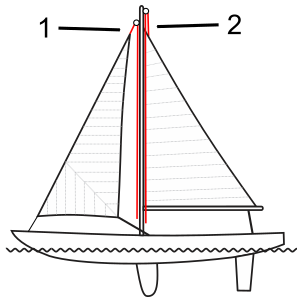
\includegraphics[width=\linewidth]{img/Halyard}
  \caption{1907 Franklin Model D roadster. Photograph by Harris \&
    Ewing, Inc. [Public domain], via Wikimedia
    Commons. (\url{https://goo.gl/VLCRBB}).}
  \Description{A woman and a girl in white dresses sit in an open car.}
\end{figure}

so important, please see
\url{https://www.acm.org/publications/taps/describing-figures/}.

\section{Citations and Bibliographies}

\begin{acks}
    Thanks is due to Dr. Kimball Germane of Brigham Young University, Provo,
    Utah for previewing drafts and offering feedback.
\end{acks}

\bibliography{\jobname}
\bibliographystyle{ACM-Reference-Format}

\end{document}
\endinput
%%
%% End of file `sample-sigconf-authordraft.tex'.
